\documentclass[technicalreport]{ieicej}
\usepackage[dvipdfmx]{graphicx,xcolor}
\usepackage[fleqn]{amsmath}
\usepackage{newtxtext}
\usepackage[varg]{newtxmath}
\usepackage{latexsym}
\usepackage{url}
\usepackage{booktabs} % 表の品質向上のため追加
\usepackage{cite}

\setcounter{page}{1}

\field{D} % 情報・システム
\jtitle{鳥獣害対策に向けた階層型エッジAI監視システムの設計と評価}
\etitle{Design and Evaluation of a Hierarchical Edge AI Monitoring System for Wildlife Damage Mitigation}
\authorlist{%
 \authorentry{佐藤 光汰}{Kota Sato}{aff1}\MembershipNumber{}
 \authorentry{伊東 峻吾}{Shungo Ito}{aff1}\MembershipNumber{}
 \authorentry{単 麟}{Lin Shan}{aff1}\MembershipNumber{}
 \authorentry{松尾 大輔}{Daisuke Matsuo}{aff1}\MembershipNumber{}
 \authorentry{佐藤 真平}{Shimpei Sato}{aff1}\MembershipNumber{}
}
\affiliate[aff1]{信州大学工学部\\ 〒380-8553 長野県長野市若里4-17-1\\ E-mail: xxxx@gmail.com}{Faculty of Engineering, Shinshu University\\ 4-17-1 Wakasato, Nagano, 380-8553 Japan}

\begin{document}
\begin{abstract}
  近年，野生鳥獣による農作物被害は深刻な社会問題となっており，ICTを活用した効率的な監視システムの構築が急務である．
  現状の主力であるPIRセンサを用いた自動撮影カメラ（トレイルカメラ）は，風による植生の揺れや気温変化に起因する誤検知（False Positive）が頻発し，通信コストの増大や画像選別の人的労力が課題となっている．
  本論文では，これらの課題解決に向け，低消費電力な撮影ノードと高機能な解析ノードを組み合わせた「階層型エッジAI監視システム」を提案する．
  本システムは，撮像と転送に特化した省電力エッジカメラ（ESP32）と，深層学習による画像選別を行うエッジサーバ（Raspberry Pi）から構成される．
  エッジサーバ上で物体検出モデルYOLOv8を稼働させ，動物が検出された画像のみをクラウドへ送信することで，通信量を劇的に削減する．
  実フィールドにおける実証実験の結果，誤検知の多い昼間において画像送信量を約81.2\%削減し，システム全体の通信コストおよび運用労力を大幅に改善可能であることを示した．
  また，システム全体の遅延は約22秒に抑えられており，鳥獣害対策に求められる即時性を損なうことなく効率化を実現した．
\end{abstract}

\begin{keyword}
  鳥獣害対策, エッジAI, IoT, 画像認識, 省電力通信
\end{keyword}

\begin{eabstract}
  This paper proposes a hierarchical edge AI monitoring system designed to mitigate agricultural damage caused by wildlife.
  Conventional camera traps largely rely on Passive Infrared (PIR) sensors, which suffer from high false-positive rates due to environmental disturbances, leading to excessive communication costs and labor-intensive image sorting.
  To address these issues, we developed a system comprising low-power edge cameras (ESP32) for image capture and transmission, and an edge server (Raspberry Pi) for intelligent filtering.
  By deploying the YOLOv8 object detection model on the edge server, the system selectively transmits only images containing animals to the cloud.
  Field experiments demonstrated an 81.2\% reduction in image transmission during daytime operation, significantly lowering communication overhead and operational effort.
  Furthermore, the total system latency was maintained at approximately 22 seconds, ensuring the real-time responsiveness required for effective wildlife management.
\end{eabstract}

\begin{ekeyword}
  Wildlife Monitoring, Edge AI, IoT, Object Detection, Low-Power Communication
\end{ekeyword}

\maketitle

\section{まえがき}
野生鳥獣による農作物被害は，日本の農業において看過できない課題である．
農林水産省の統計によれば，令和5年度の被害総額は約180億円に達しており，経済的損失のみならず，営農意欲の減退や耕作放棄地の拡大といった副次的な被害をもたらしている\cite{maff}．
効果的な鳥獣害対策を立案・実行するためには，対象動物の出没状況を正確かつリアルタイムに把握するモニタリング体制の構築が不可欠である．

従来，この目的にはPIR（Passive Infrared Ray）センサを搭載したトレイルカメラが広く利用されてきた．
しかし，既存のトレイルカメラシステムは，運用面における重大な技術的課題を抱えている．
第一に，PIRセンサの誤検知（False Positive）による「空画像」の大量発生である．
PIRセンサは背景温度との差分を検知するため，風による草木の揺れや日射による地面の急激な温度上昇にも反応しやすく，動物が写っていない画像を大量に撮影・送信してしまう．
これにより，管理者は数千枚に及ぶ画像の中から動物が写っている画像を目視で選別する必要があり，看過できない人的コストが発生する．
第二に，ランニングコスト（通信費）の増大である．
LTE回線を利用したリアルタイム監視を行う場合，送信データ量の増加は通信料金に直結する．
特に誤検知による不要な画像の送信は，予算の限られた自治体や個人農家にとって大きな負担となる．

本論文では，これらの課題に対する工学的解として，処理機能を分散・階層化した「低コスト通信型警戒システム」を提案する．
提案システムは，撮像機能に特化した複数の安価な「エッジカメラ」と，高度な画像処理能力を持つ「エッジサーバ」を連携させるアーキテクチャを採用する．
エッジサーバが集約ゲートウェイとして機能し，深層学習モデルを用いて画像の選別を行うことで，クラウドへの送信データを真に重要な情報のみに限定する．
これにより，通信コストの削減，画像確認労力の軽減，およびシステム全体の省電力化を同時に達成することを目的とする．

\section{関連研究とその課題}
野生動物モニタリングの自動化・効率化に向け，近年では深層学習（Deep Learning）の応用が活発に研究されている．
Tabakら\cite{Tabak2019}は，大規模データセットで学習したCNN（Convolutional Neural Networks）を用いることで，カメラトラップ画像から動物種を高精度に識別可能であることを示した．
また，Fennellら\cite{Fennell2022}は物体検出技術を用いて動物と人間を区別し，プライバシー配慮型の調査手法を提案している．
しかし，これらの多くはSDカード回収後の事後解析や，全画像をクラウドへアップロードした後のサーバサイド処理を前提としており，通信帯域が狭く，かつ即時通知が求められる鳥獣害対策の現場要件とは必ずしも合致しない．

即時性を追求したシステムとして，Whytockら\cite{Whytock2023}は衛星通信を用いたリアルタイムアラートシステムを開発したが，高額な通信コストが導入の障壁となる．
一方，エッジコンピューティングのアプローチとして，Patkarら\cite{Patkar2025}やRahmanら\cite{Computers2025}は，Raspberry Pi等のシングルボードコンピュータを各観測地点に配置する手法を提案している．
これらのシステムは高度な処理が可能であるが，デバイス単体の消費電力が大きく，商用電源のない環境では大型の太陽光発電システムが必要となり，設置コストとメンテナンス性を悪化させる要因となる．

省電力化のアプローチとして，Saitoら\cite{IEICE2020}はESP32等のMC (Micro Controller) 上での軽量モデル推論を検討しているが，計算リソースの制約から認識精度や処理速度に限界があり，複雑な環境下での実用性には課題が残る．

本研究の独自性は，これらのトレードオフを解消するために「階層型アーキテクチャ」を採用した点にある．
極低消費電力なマイコンベースの撮影ノードと，十分な計算資源を持つ集約ノードを分離・連携させることで，全体としての「低コスト性」「省電力性」と「高機能性」の両立を図る．

\section{提案システム}

\subsection{システムアーキテクチャ}
提案システムの全体構成を図\ref{fig:system}に示す．本システムは以下の3層構造を有する．
\begin{enumerate}
  \item \textbf{Sensor Layer (Edge Camera)}: 画像収集と近距離転送を担当．
  \item \textbf{Processing Layer (Edge Server)}: データ集約，推論処理，クラウド連携を担当．
  \item \textbf{Application Layer (Cloud Server)}: データ蓄積，ユーザ通知，可視化を担当．
\end{enumerate}

\begin{figure}[tb]
  \centering
  \framebox[80mm][c]{\rule{0pt}{50mm}System Configuration Diagram}
  \caption{提案システムの全体構成}
  \label{fig:system}
\end{figure}

\begin{figure*}[tb]
  \centering
  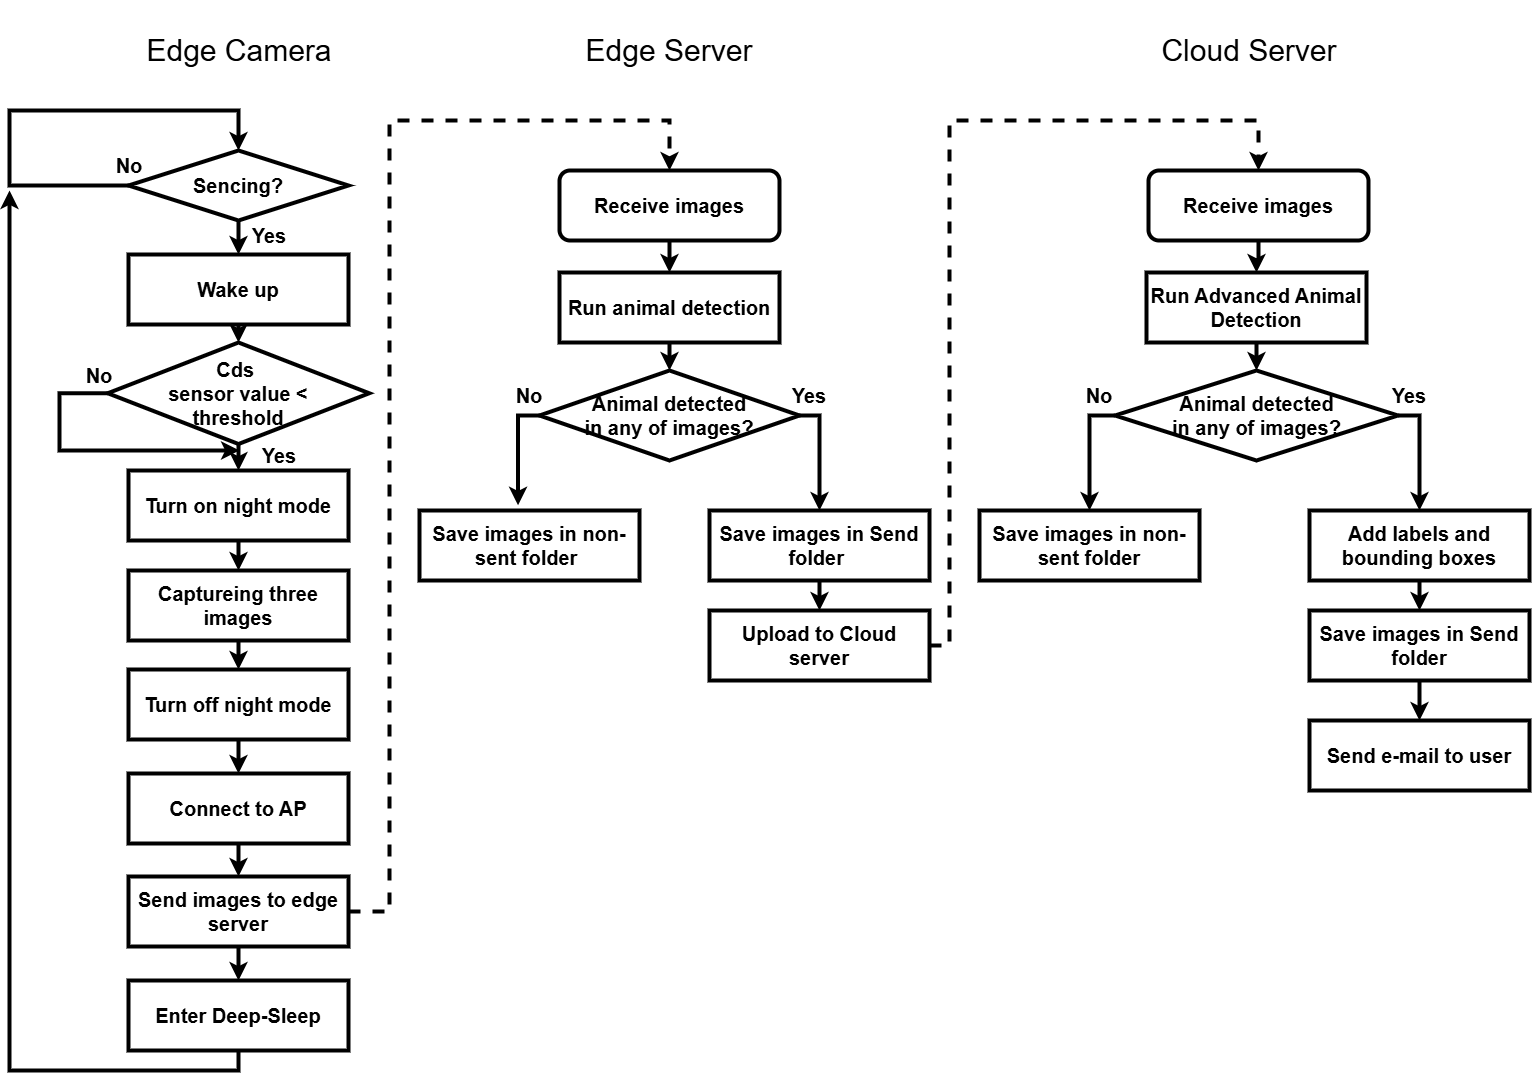
\includegraphics[width=0.85\linewidth]{img/system_flow.png}
  \caption{提案システムの処理フロー}
  \label{fig:flow}
\end{figure*}

この構成により，広範囲に展開する多数のカメラノードは安価かつ最小限の機能で構成し，高価な計算リソースや通信モジュールをサーバノードに集約することが可能となる．

\subsection{構成要素の実装}
\subsubsection{エッジカメラ (Edge Camera)}
エッジカメラには，Seeed Studio製のXIAO ESP32S3 Senseを採用した（図\ref{fig:camera}）．
本デバイスはWi-Fiおよびカメラ機能を内蔵しながら，Deep Sleep時の消費電力が極めて低い特性を持つ．
電源には入手性の高い単3電池8本を使用し，特別な電源工事を不要とした．

動作フローは以下の通りである．
\begin{enumerate}
  \item PIRセンサによる熱源検知によりDeep Sleepから復帰．
  \item バースト撮影（連続3枚）を実行．
  \item Wi-Fi（HTTP POST）を用いて画像をエッジサーバへ送信．
  \item 送信完了後，直ちにDeep Sleepモードへ移行．
\end{enumerate}
この「撮って送って寝る」という単純な動作に徹することで，バッテリー寿命の最大化を図っている．

\subsubsection{エッジサーバ (Edge Server)}
エッジサーバは監視エリア内のゲートウェイとして機能する．
計算機としてRaspberry Pi 4Bを使用し，電源には10Wソーラーパネルと25Ahバッテリー（Hyke Solar Power Pack）を組み合わせた独立電源システムを採用した．
通信モジュールにはLTEルータ（NEC Aterm HT100LN）を用い，インターネット接続性を確保している．

ソフトウェア面では，物体検出モデルとしてYOLOv8 Nano (YOLOv8n) を採用した．
受信した画像に対してCOCOデータセットで学習済みのモデルにより推論を行い，検出されたクラスに動物（Bird, Cat, Dog, Bear, Sheep, Cow, Horse等）が含まれる場合のみ，画像を保存・転送対象とする．
動物が含まれないと判定された画像は，誤検知として即座に破棄される．

\subsubsection{クラウドサーバ (Cloud Server)}
クラウド側では，受信画像のアーカイブとユーザへの通知を行う．
本研究のスコープはエッジ側の最適化にあるため，クラウド側の機能は基本的な通知機能（LINE/メール連携）の実装に留めるが，将来的な拡張としてより大規模なモデル（MegaDetector等）による二次解析を行うことも可能である．

\begin{figure}[tb]
  \centering
  \framebox[80mm][c]{\rule{0pt}{50mm}Edge Camera Prototype}
  \caption{エッジカメラのプロトタイプ}
  \label{fig:camera}
\end{figure}

\section{実験データによる評価}
提案システムの有効性を検証するため，長野県内の山林フィールドにおいて運用試験を実施した．
評価の主眼は「通信削減効果」と「実用上の信頼性」におく．

\subsection{実験環境}
表\ref{tab:components}に実験機材の仕様を示す．
エッジカメラは野生動物の獣道に向けて設置し，エッジサーバはそこからWi-Fi通信可能な範囲（約5--10m）に配置した．

\begin{table}[tb]
  \caption{実験機材の仕様}
  \label{tab:components}
  \centering
  \begin{tabular}{l|l}
    \hline
    Component            & Specification                  \\
    \hline \hline
    \textbf{Camera Node} & XIAO ESP32S3 Sense (OV2640)    \\
    MCU                  & Xtensa LX7 (240MHz)            \\
    Power                & AA Batteries $\times$ 8        \\
    \hline
    \textbf{Server Node} & Raspberry Pi 4B (4GB RAM)      \\
    Power                & 10W Solar + 25Ah Battery       \\
    Connectivity         & Wi-Fi (Local) + LTE (Backhaul) \\
    \hline
  \end{tabular}
\end{table}

\subsection{消費電力特性}
エッジカメラの持続可能性を評価するため，各動作フェーズの消費電流を測定した（表\ref{tab:camera_power}）．
Deep Sleep時の消費電力は0.585mWであり，これは長期間の待機運用において極めて有利な特性である．
1日あたりの撮影回数をXX回と仮定した場合，理論上の稼働期間は約XXヶ月と試算され，頻繁な電池交換を必要としない実用的な省電力性を確認した．

\begin{table}[tb]
  \caption{エッジカメラの消費電力（実測値）}
  \label{tab:camera_power}
  \centering
  \begin{tabular}{l|c|c|c}
    \hline
    State        & Voltage (V) & Current ($\mu$A) & Power (mW) \\
    \hline \hline
    Deep Sleep   & 5.0         & 117              & 0.585      \\
    Active (Avg) & 5.0         & XXX.X            & XXXX.X     \\
    Wi-Fi Tx     & 5.0         & XXX.X            & XXXX.X     \\
    \hline
  \end{tabular}
\end{table}

\subsection{AIフィルタリング性能と通信削減効果}
本システムの核心である画像選別機能の精度を定量評価した．
実験期間中に得られた全トリガー画像に対し，目視確認による正解ラベル（Ground Truth）を作成し，システム（YOLOv8n）の判定結果と比較した．
表\ref{tab:ai_accuracy}に混同行列および精度指標を示す．

\begin{table}[tb]
  \caption{推論精度および再現率の評価（閾値0.05）}
  \label{tab:ai_accuracy}
  \centering
  \begin{tabular}{l|rr}
    \hline
    指標        & 夜間 (Night) & 昼間 (Day) \\
    \hline \hline
    TP (正検知)  & 104        & 195      \\
    FP (誤検知)  & 28         & 73       \\
    FN (見逃し)  & 48         & 13       \\
    TN (正棄却)  & 88         & 1147     \\
    \hline
    Precision & 78.8\%     & 72.8\%   \\
    Recall    & 68.4\%     & 93.8\%   \\
    Miss Rate & 31.6\%     & 6.2\%    \\
    \hline
  \end{tabular}
\end{table}

特筆すべきは昼間のTrue Negative（TN）数である．
昼間は1428回のトリガーが発生したが，そのうち1147回は動物の写っていない誤作動画像であった．
システムはこれらを正しく「動物なし」と判定し，送信を抑制している．
表\ref{tab:comm_reduction}に示す通り，昼間の通信削減率は81.2\%に達した．
これは，従来システムであれば無駄に送信されていたデータの大半をカットできたことを意味し，通信コスト削減に対する本提案の貢献は著しい．

\begin{table}[tb]
  \caption{フィルタリングによる通信削減率}
  \label{tab:comm_reduction}
  \centering
  \begin{tabular}{l|rr}
    \hline
    項目       & 夜間 (Night) & 昼間 (Day) \\
    \hline \hline
    全検知回数    & 268        & 1428     \\
    送信回数     & 132        & 268      \\
    削減率 (\%) & 50.7       & 81.2     \\
    \hline
  \end{tabular}
\end{table}

一方，夜間のRecallは68.4\%に留まった．
これは暗所における画質低下や，赤外線照射範囲の限界により，小型動物の識別が困難であったためと考えられる．
しかし，鳥獣害対策においては「明らかな誤検知を排除すること」がコスト面で最重要視される傾向にあり，Precisionを維持しつつ50\%以上の不要通信を削減できた点は評価に値する．

\subsection{システム応答性}
エッジ側で画像処理を行うことによる遅延の影響を調査した．
カメラでの撮影からユーザへの通知完了までの総所要時間は平均約21.9秒であった（表\ref{tab:latency}）．
この遅延にはWi-Fi接続やLTE通信のオーバーヘッドが含まれるが，数十分〜数時間のタイムラグが発生する定期送信型システムと比較すれば十分に「リアルタイム」と呼びうる範囲である．

\begin{table}[tb]
  \caption{処理フェーズごとの所要時間}
  \label{tab:latency}
  \centering
  \begin{tabular}{l|r}
    \hline
    処理フェーズ                 & 時間 (ms)        \\
    \hline \hline
    画像撮影 (Capture)         & 3105           \\
    Wi-Fi転送 (Transmission) & 7991           \\
    推論処理 (Inference)       & 3241           \\
    クラウド通知 (Notification)  & 7651           \\
    \hline
    \textbf{合計 (Total)}    & \textbf{21988} \\
    \hline
  \end{tabular}
\end{table}

\section{むすび}
本論文では，鳥獣害対策の現場課題である「センサ誤検知による通信コスト増大」を解決するため，階層型エッジAI監視システムを設計・構築した．
実証実験において，本システムは特に誤検知の多発する昼間環境下で81.2\%の画像送信量を削減することに成功した．
これにより，運用コストを最小限に抑えつつ，必要な情報を確実に管理者に届けることが可能となった．
また，エッジカメラの徹底的な省電力化により，電源インフラに依存しない柔軟な設置運用性を実証した．

今後の展望として，夜間認識精度の向上に向けたモデルの最適化（センサフュージョンやドメイン適応），およびLPWA技術の導入による通信カバレッジの拡張に取り組む予定である．

\ack
本研究の一部は，XXXXXの助成を受けて行われた．

\bibliographystyle{sieicej}
\bibliography{refs}

\end{document}
